\section{The Standard Model of Particle Physics}
The Standard Model (SM) of particle physics classifies the elementary particles, as well as three of the four fundamental forces of nature \cite{oerter2006theory}. 
These forces include electromagnetism, the weak interaction, and the strong interaction.
The nature by which these fundamental facets of the universe interact is described through the mathematical formalisms of quantum field theory.
Unfortunately, a complete quantum field theory of gravity is not yet known, however, efforts continue in the pursuit of combining Einstein's General Relativity with quantum mechanics.
Despite this missing piece the SM continues to have theoretical predictions validated by experimental evidence.

The particles of the SM are represented as excitations of quantum fields.
Matter particles - the quarks and leptons - are described by fermion fields, characterised by having half-integer spin values.
The field dynamics of which are described by their Lagrangian, $\mathcal{L}$, a quantity that describes the kinematics and excitations of the particular field. 
The complete Lagrangian for the SM as a whole must obey certain symmetries, including translational and rotational symmetries, as well as the inertial frame invariance prescribed by special relativity.
Furthermore, a local $SU(3) \times SU(2) \times U(1)$ gauge symmetry must be obeyed to ensure the renormalisabielity of the theory. 
Without the ability to be renormalised, the SM would not possess the predictive capability is has.
In order to preserve the gauge invariance, inclusion of gauge fields with integer spin must be included.
These integer spin fields are the so-called boson fields, and they describe particles that carry the three forces included in the SM.
From this we get, in total, twelve gauge fields required to write a gauge invariant SM Lagrangian, one from the single $U(1)$ generator, three for the $SU(2)$ generators, and eight for the $SU(3)$ generators.
In conjunction with nineteen numerical constants, given in table \ref{tab:parameters}, we are furnished with the ability to write down a gauge invariant SM Lagrangian

\subsection{The Electroweak Interaction}
\label{subsec:EWInteraction}
The Electroweak theory \cite{glashow1959renormalizability} describes the unification of the electromagnetic and weak interactions, described mathematically by an $SU(2) \times U(1)$ gauge symmetry.
Electroweak theory introduces two complications to the SM.
As stated previously, four gauge fields are included from the $SU(2)$ and $U(1)$ gauges, however, to preserve gauge invariance they are required to be massless.
This is a direct contradiction to experimental evidence which shows that the weak force carriers, the $W^{\pm}$ and $Z^{0}$ bosons, are massive.
Furthermore, the weak interaction couples differently to different fermion helicity states.
The solution to this is to treat the two helicity states as different fields with different couplings, however, to preserve gauge invariance fermions would have to also be massless.
Again, this is in direct contradiction with observation.

The solution to both problems is to introduce to concept of spontaneous symmetry breaking. 
Essentially, spin-0 scalar fields are introduced that couple to the electroweak gauge fields and preserve the gauge invariance of the Lagrangian.
The new interaction potentials are chosen in such a way that the field's lowest energy states do not correspond with the field's zero values.
Therefore, the field's ground state will break the $SU(2) \times U(1)$ symmetry, while the Lagrangian simultaneously preserves the symmetry.
These scalar fields acquire non-zero values, named the vacuum expectation value (VEV), which allows for the fermion fields and weak interaction gauge bosons to be massive particles.
A consequence of this mechanism is that one extra scalar field obtains mass, therefore a neutral spin-0 massive particle is predicted to exist; the Higgs boson.

With this mechanism one can write the electroweak Lagrangian as follows:
\begin{align}
\mathcal{L}_{EW} = \mathcal{L}_{\textrm{gauge}} + \mathcal{L}_{\textrm{fermion}} + \mathcal{L}_{\textrm{Higgs}} + \mathcal{L}_{\textrm{Yukawa}}.
\end{align}

\noindent In the gauge portion of the Lagrangian we obtain an isotriplet from the $SU(2)$, written as $\textbf{W}^{\mu}_{1,2,3}$, and a singlet from the $U(1)$, $B^{\mu}$.
From this, one write the gauge term as
\begin{align}
\mathcal{L}_{\textrm{gauge}} = -\frac{1}{4}\left(\textbf{W}^{\mu \nu}W_{\mu \nu} + B^{\mu \nu}B_{\mu \nu} \right),
\end{align}
where
\begin{align}
\textbf{W}^{\mu \nu} = \partial^{\mu} \textbf{W}^{\nu} - \partial^{\nu} \textbf{W}^{\mu} - g_{2} \textbf{W}^{\mu} \times \textbf{W}^{\nu}
\end{align}
and
\begin{align}
B^{\mu \nu} = \partial^{\mu} B^{\nu} - \partial^{\nu} B^{\mu}
\end{align}
where $g_{2}$ is the $SU(2)$ gauge coupling constant.
The $Z^{0}$ boson and photon are generated by the superposition of the $W_{3}$ and $B$ fields as follows:
\begin{align}
\begin{pmatrix}
\gamma \\
Z^{0}
\end{pmatrix} = \begin{pmatrix} 
\cos\theta_{W} & \sin\theta_{W} \\
-\sin\theta_{W}& \cos\theta_{W} 
\end{pmatrix} \begin{pmatrix}
B \\
W_{3}
 \end{pmatrix}.
\end{align}
Here, $\theta_{W}$ is the weak mixing angle defined using the ratio of weak boson masses:
\begin{align} 
\cos\theta_{W} = \frac{M_{W}}{M_{Z}}
\end{align}
where $M_{W}$ and $M_{Z}$ are the $W$ and $Z$ boson masses respectively.
Similarly, the $W^{\pm}$ bosons are defined through a superposition of the $W_{1}$ and $W_{2}$ fields as follows:
\begin{align}
W^{\pm} = \frac{1}{\sqrt{2}} \left(W_{1} \mp iW_{2} \right).
\end{align}
The fermion portion of the Electroweak Lagrangian is given as
\begin{align}
\mathcal{L}_{\textrm{fermion}} = i \bar{\psi}\slashed{D}\psi
\end{align}
with the covariant derivative for electroweak theory defined as 
\begin{align}
D_{\mu} =  \partial_{\mu} + ig_{2}\textbf{W}_{\mu} \cdot \textbf{T} + \frac{1}{2} ig_{1} B_{\mu} Y,
\label{eqn:EWDerivative}
\end{align}
where $\textbf{T}$ is the weak isospin, $g_{1}$ is the $U(1)$ gauge coupling, and $Y$ is the weak hypercharge. \textit{potentially define these terms}
The Higgs component of the Electroweak Lagrangian is defined as 
\begin{align}
\mathcal{L}_{\textrm{higgs}} = \left| D_{\mu} h \right| -\lambda \left( \left| h \right|^{2} - \frac{v^{2}}{2} \right)^{2},
\end{align}
where $v$ is the VEV and $D_{\mu}$ is as given in equation \ref{eqn:EWDerivative}. 
The mass of the Higgs boson was observed in 2012 by ATLAS and CMS, and is recorded to have a mass of $m_{h} = 125.09 \pm 0.24$ GeV \cite{aad2012observation, chatrchyan2012observation}.
Finally, the Yukawa interaction which describes the interaction between fermions and the Higgs field is given by
\begin{align}
\mathcal{L}_{\textrm{Yukawa}} = \sum -\lambda_{e} \bar{L} h e_{R} - \lambda_{d} \bar{Q} h d_{R} - \lambda_{u} \epsilon^{ab}\bar{Q}_{a} h^{\dagger}_{b} u_{R} + h.c.
\end{align}
where $\lambda_{x}$ is the Yukawa coupling for a particular fermion, $x$, $L$ and $e_{R}$ and the lepton fields, $Q$, $u_{R}$, and $d_{R}$ and the quark fields, and $\epsilon$ is the rank two Levi-Civita symbol.

\subsection{Quantum Chromodynamics}
The theoretical description of the strong force is described by Quantum Chromodynamics (QCD), underlined by the $SU(3)$ gauge symmetry. 
As stated previously, eight gauge fields are associated with $SU(3)$ which correspond to different coloured states of the strong force boson, the gluon.

The Lagrangian for QCD is given as
\begin{align}
\mathcal{L}_{\textrm{QCD}} = - \frac{1}{4}G^{a}_{\mu \nu} G^{\mu \nu}_{a} + \bar{\psi}_{i}\left(i \left(\gamma^{\mu}D_{\mu}\right)_{ij} - m\delta_{ij}\right)\psi_{ij} 
\label{eqn:strongLagrangian}
\end{align}
where $G^{a}_{\mu \nu}$ is the QCD field strength tensor, given as
\begin{align}
G^{a}_{\mu \nu} = \partial_{\mu} A_{\nu}^{a} - \partial_{\nu} A_{\mu}^{a} + g_{3} f^{abc} A_{\mu}^{b} A_{\nu}^{c},
\end{align}
where $A_{\mu}^{a}(x)$ are the gluon fields as a function of four dimensional spacetime, $f^{abc}$ are the structure constants of the $SU(3)$ gauge group, $m$ is the quark mass, and $g_{3}$ is the $SU(3)$ gauge coupling constant.
The covariant derivative in QCD is given as
\begin{align}
D_{\mu} = \partial_{\mu} + ig_{3} \frac{\lambda^{a}}{2} G_{\mu}^{a}
\end{align}
where $\lambda^{a}$ are the eight Gell-Mann  matrices. 
Within equation \ref{eqn:strongLagrangian}, the index $i$ runs from 1-3 to cover the three colour charges: red, green, and blue.
It is important to note that, for example, if one has up quark of colour charge red, the corresponding antiquark will have colour charge anti-red.
This is analogous to electromagnetism where the electric charge of an anti-particle is the negative of the charge of a normal particle.
The indices that run over the gluon field, a, b, c, run from 1-8, corresponding to the eight colour charge combinations.
A visual representation of the quark and gluon colour charge combinations is given in figure \ref{fig:colourCharge}.

\begin{figure}[H] %  figure placement: here, top, bottom, or page
   \centering
   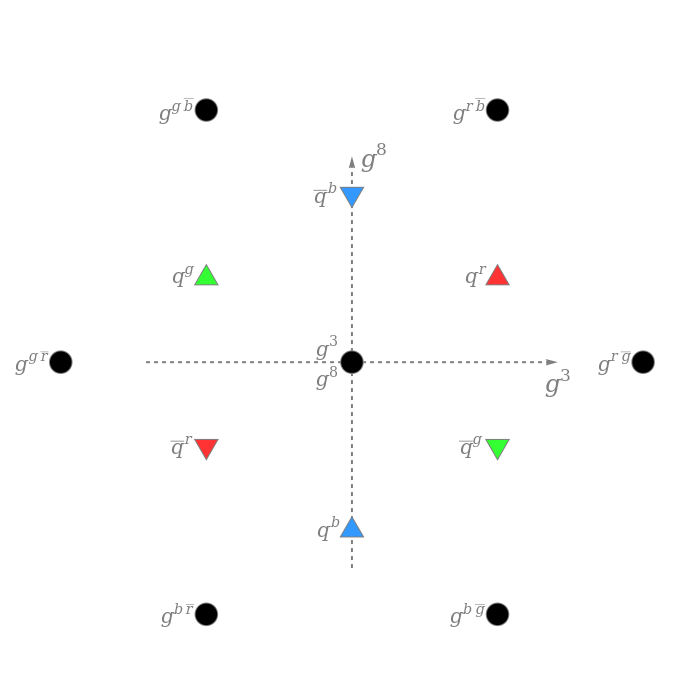
\includegraphics[width=.5\textwidth]{Pictures/SU(3).png} 
   \caption{A visual representation of the colour charge combinations allowed for quarks and gluons}
   \label{fig:colourCharge}
\end{figure}

\noindent It is important that, similarly to electric charge, colour charge must be conserved in strong interactions.

With the catalogue of theory describing the strong interaction, QCD has become another success of the SM.
The existence of gluons has been inferred by experiment.
Furthermore, their interaction with quarks is consistent with that described in the theory \cite{brandelik1979evidence}.

\subsection{Limits of the Standard Model}
The SM has been rigorously tested for several decades, with predictions closely matching experimental results.
However, the SM is not without its shortcomings, the most obvious of which is the lack of an explanation of gravity.
Currently, the inclusion of terms involving gravity leads to the inability of the theory to be renormalised.
Without renormalisabielity, the theory loses the ability to make qualified predictions. 
Luckily, the energy regime in which gravitational effects are noticeable is far beyond our current capabilities.
For gravitational effects to be important experiments would need to be approaching the Planck energy, defined as
\begin{align}
E_{\textrm{Planck}} = \sqrt{\frac{\hbar c^{5}}{G_{N}}} \approx 1.2 \times 10^{16}\ \textrm{TeV}
\end{align}
\cite{ade2014planck}. 
By comparison, the LHC at CERN reaches energies of $\sqrt{s} = 13$ TeV, fifteen orders of magnitude smaller than the Planck energy.

Other big questions in physics include:
\begin{itemize}
\item Matter-antimatter asymmetry: Naturally occurring antimatter is effectively nonexistent, minimally coming from cosmic ray interactions. 
The asymmetry is thought to come from $CP$-violating interactions, where $CP$ is the combined symmetry of charge conjugation ($C$) and parity conservation ($P$).  
Although there are $CP$-violating terms in the quark mixing and neutrino mixing matrices, these terms are not large enough to compensate for the matter-antimatter disparity \cite{canetti2012matter}.

\item Neutrino masses: When observing solar neutrinos, it is seen that neutrinos undergo flavour change. 
This effect is known as neutrino oscillations and immediately implies that neutrinos have mass.
This observation is contradictory to the SM which predicts massless neutrinos \cite{olive2014review}.

\item Dark matter: Cosmological observations of the motion and masses of galaxies cannot be reconstructed from the visible matter.
It is theorised that there is a substance, named "Dark Matter", that is massive and doesn't interact electromagnetically, thereby being invisible.
Currently, there is no definitive dark matter candidate from the SM \cite{bertone2005particle}. 
\end{itemize}
These limitations are but a few of the unexplained factions of nature that need to be overcome by expanding our physical theories.
Such expansions come in the forms of new particles and particle interactions, however, it is not known at what energies new physical effects would manifest themselves.
For this we must explore the two energy regimes of nature: the electroweak scale $\mathcal{O}(10^{2})$ GeV, and the Planck scale, $\mathcal{O}(10^{19})$ GeV.
Since we know that the SM is accurate at low energies and has the ability to be normalised it should theoretically have predictive capabilities at higher energies.
This inherently works against the theory, however, as illustrated by calculating the mass of the Higgs boson.
One can express the physical mass of the Higgs boson as 
\begin{align}
m_{\textrm{h, physical}}^{2} \approx m_{h}^{2} + \delta m_{h}^{2}
\end{align}
where $m_{h}$ is the Higgs mass parameter in the Higgs Lagrangian, and $\delta m_{h}$ are the first order corrections to the Higgs mass.
These corrections include those shown in figure \ref{fig:HiggsCorrections}

\begin{figure}[H]
    \centering
    \begin{subfigure}[b]{0.33\textwidth}
        \centering
        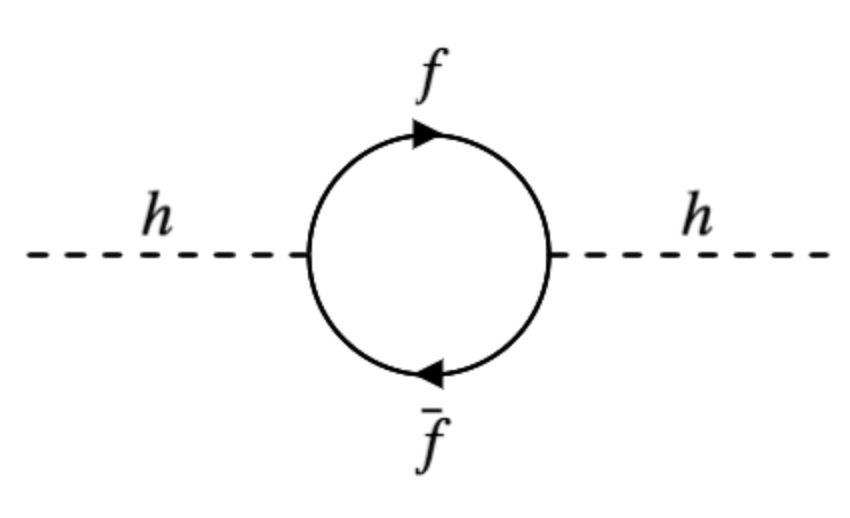
\includegraphics[width=\textwidth]{../Pictures/HiggsFermionCorr.png}
        \caption{}
        \label{fig:FermionCorrection}
    \end{subfigure}
    ~
    \begin{subfigure}[b]{0.33\textwidth}
        \centering
        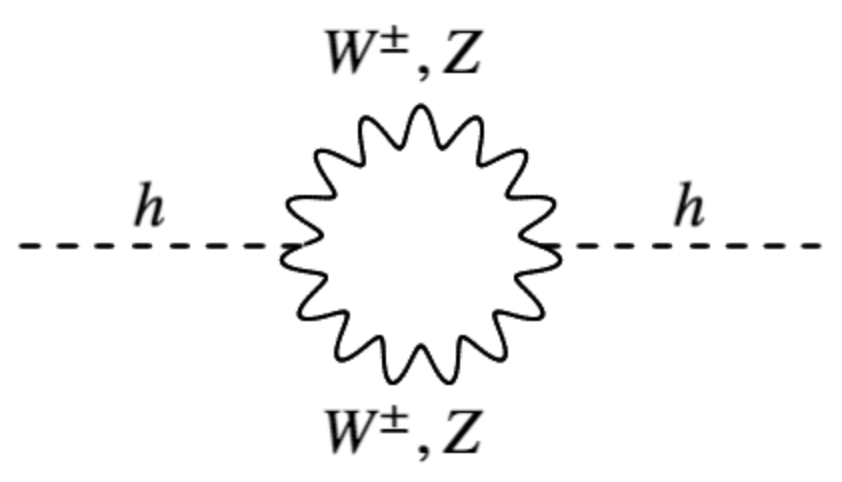
\includegraphics[width=\textwidth, height=1.5in]{../Pictures/HiggsGaugeCorr.png}
	\caption{}
	\label{ref:BosonCorrection}
    \end{subfigure}
        ~
    \begin{subfigure}[b]{0.33\textwidth}
        \centering
        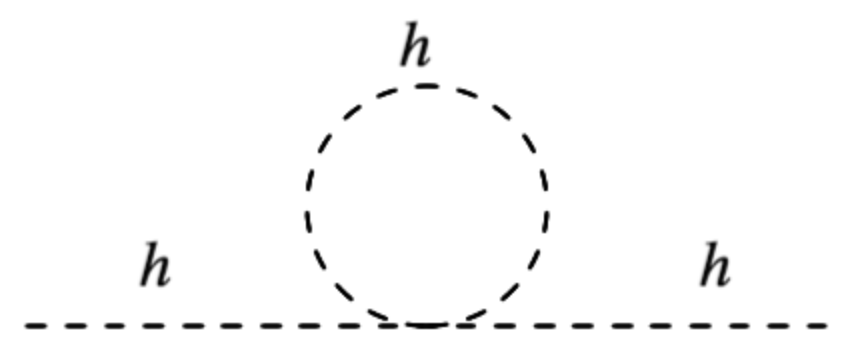
\includegraphics[width=\textwidth]{../Pictures/HiggsHiggsCorr.png}
        \caption{}
    \end{subfigure}
    \caption{Loop corrections from (a) fermions, (b) $W$ and $Z$ bosons, and (c) the Higgs bosons in the mass calculation of the Higgs boson}
    \label{fig:HiggsCorrections}
\end{figure}

\noindent With a full quantum field treatment one is able to express the Higgs mass as
\begin{align}
m_{\textrm{h, physical}}^{2} \approx m_{h}^{2} + \frac{C}{16 \pi} \Lambda^{2}
\end{align}

where $C$ is an amalgamation of SM coupling constants.
A full breakdown is given in \cite{baer2015supergravity}.
The issue that arises is that when calculating the parameter $\Lambda$, quantum corrections pile up causing $\Lambda$ to be of the order of the Planck scale.
The result of this is that the Higgs mass is predicted to be of the order of the Planck scale, whereas experiment shows that it is actually of the order of the electroweak scale; a difference of seventeen orders of magnitude.
The immediate solution to this is to "tune" the parameter $m_{h}$ in such a way that it cancels out the substantial $\Lambda$ correction.
Ultimately, this tuning requirement implies that the SM is essentially a low-energy solution to nature,  accurate to an energy of $\Lambda \sim \mathcal{O}(1)$ TeV.
Fortuitously, this is the energy regime in which current colliders are able to operate, therefore we are able to explore, and hopefully discover, new physics at the boundary of the SM.

\section{Supersymmetry}
Limitations of the SM, such as the previously discussed Higgs mass problem, can be alleviated by introducing a symmetry between matter particles and gauge bosons.
By imposing this link between bosons and fermions figures \ref{fig:HiggsCorrections}\subref{fig:FermionCorrection} and \ref{fig:HiggsCorrections}\subref{ref:BosonCorrection}'s weights could balance one another in calculating the mass of the Higgs boson. 
This, in turn, would bring the final result back down to the value we acquire experimentally.
It is this new symmetry that is given the name \textit{supersymmetry} (SUSY).
Additionally, SUSY offers a promising dark matter candidate as well as a new family of particles, searches for which are currently highly active and the LHC at CERN.

\subsection{Theoretical Overview of Supersymmetry}
Within the SM the symmetries we experience are usual space-time symmetries: translations, rotations, and boosts.
Furthermore, we have the $SU(3) \times SU(2) \times U(1)$ symmetry group as discussed previously.
The symmetries of the SM allow for the transformation of a neutron to a proton, however, it does not allow for the transformation of a neutron to a pion.
The important quantity that must be considered here is the spin value of the given particles.
Neutrons and protons are both spin-1/2 fermions, whereas pions are spin-0 bosons.
Conversely, as supersymmetry provides a link between integer and half-integer spin particles, it would be possible for a transformation of a fermion to a boson, and vice versa.

Mathematically, the generation of supersymmetric states is done by use of the four generators: $Q_{\alpha}$, $Q_{\dot{\alpha}}$, $\overline{Q}_{\alpha}$, and $\overline{Q}_{\dot{\alpha}}$. 
Here $\alpha$ and $\dot{\alpha}$ represent the left and right-handed Weyl spinor indices respectively, and $Q$ and $\overline{Q}$ are the particle and anti-particle states respectively.
These generators can act on a scalar state, as follows
\begin{align}
Q_{\alpha} \left| \phi \right> = \left|\psi_{\alpha}\right>,
\end{align}
producing a spinor containing both fermion and boson fields, often referred to as supermultiplets. 
These generated states will be either chiral-states, having a boson and a left-handed fermion, or anti-chiral, having a boson and a right-handed fermion.
As a result, if supersymmetry is in fact an extension to the SM, it implies that for every particle there exists a supersymmetric partner with identical quantum numbers and a spin value that differs by one half.

Within the formalisms of supersymmetry one finds 
\begin{align}
\left[Q, P^{\mu} \right] = 0,
\end{align}
where $Q$ is the SUSY generator operator and $P^{\mu}$ is the momentum operator.
The fact that these two operators commute implies that if supersymmetry is an exact symmetry, the fermion and boson states of the supermultiplet must have identical masses.
This, however, does not appear to be the case as no supersymmetric particles have been found to have masses similar to the masses of SM particles.
What this implies is that supersymmetry is a broken symmetry, however, this concept is not well understood yet and so models that preserve certain features of supersymmetry but still account for its breaking are being developed. 
This is known as soft supersymmetry breaking, and essentially allows for the mass splitting of SUSY partners to be up to $\mathcal{O}(1)$ TeV.
This scheme hold promise as the concept itself can be linked to electroweak symmetry breaking \cite{chung2005soft} and places SUSY partners within the mass capabilities of current experiments.

\subsection{Minimal Supersymmetric Standard Model} 
The Minimal Supersymmetric Standard Model, often referred to as the MSSM for short, is an extension to the SM that includes SUSY. 
It is minimal as it introduces the fewest number of new particles states and interactions required to be consistent with the phenomenology \cite{baer2006weak}.

Fundamentally, this model replaces SM particles with SUSY supermultiplets containing their additional fermions or bosons. 
For the sake of semantics, a nomenclature is introduced to differentiate between SM and SUSY particles.
A SM fermion, such as a quark or lepton, is paired with a SUSY particle of the same name, prefixed with `$s$-'. 
For example, the up quark ($u$) is paired with the sup squark ($\tilde{u}$).
Simillarly, SM bosons are paired with SUSY fermions of the same name, however, this time suffixed with `-$ino$', giving us the bino ($\tilde{B}$), wino ($\tilde{W}$), and gluino ($\tilde{g}$).

An important feature of the MSSM is the two Higgs doubles, $H_{u}$ and $H_{d}$, which only give mass to the up and down quarks respectively. 
Furthermore, for the MSSM to be normalised there must be at least two Higgs fields.
As a result of this we end up with four Higgs-type states, $H^{0}_{u},  H^{0}_{d}, H^{+}_{u}, H^{-}_{d}$, all of which have supersymmetric partners.

A full table of MSSM particles is given in table \ref{tab:MSSMParticles}

\begin{table}[H]
\begin{center}
\begin{tabular}{ c c c c }
\toprule
Particle Group    & Spin     & Gauge Eigenstate     & Mass Eigenstate \\
\midrule 
\vspace{3mm}
        &         & $\tilde{u}_{L}, \tilde{u}_{R}, \tilde{d}_{L}, \tilde{d}_{R}$    & same    \\
\vspace{3mm}
squarks     & $0$    & $\tilde{c}_{L}, \tilde{c}_{R}, \tilde{s}_{L}, \tilde{s}_{R}$    & same    \\
\vspace{3mm}
        &         & $\tilde{t}_{L}, \tilde{t}_{R}, \tilde{b}_{L}, \tilde{b}_{R}$    & $\tilde{t}_{1}, \tilde{t}_{2}, \tilde{b}_{1}, \tilde{b}_{2}$    \\

\hline 

\vspace{3mm}
        &         & $\tilde{e}_{L}, \tilde{e}_{R}, \tilde{\nu}_{e}$        & same    \\
\vspace{3mm}
sleptons     & $0$    & $\tilde{\mu}_{L}, \tilde{\mu}_{R}, \tilde{\nu}_{\mu}$    & same    \\
\vspace{3mm}
        &         & $\tilde{\tau}_{L}, \tilde{\tau}_{R}, \tilde{\nu}_{\tau}$    & $\tilde{\tau}_{1}, \tilde{\tau}_{2}, \tilde{\nu}_{\tau}$    \\    
        
\hline \\

gluino    & $1/2$    & $\tilde{g}$    &    same \\
\\
\hline \\

Neutralinos    & $1/2$    & $\tilde{B}^{0}, \tilde{W}^{0}, \tilde{H}^{0}_{u}, \tilde{H}^{0}_{d}$& $\tilde{\chi}^{0}_{1}, \tilde{\chi}^{0}_{2}, \tilde{\chi}^{0}_{3}, \tilde{\chi}^{0}_{4}$ \\
\\
\hline \\

Charginos        & $1/2$    & $\tilde{W}^{\pm}, \tilde{H}^{+}_{u}, \tilde{H}^{-}_{d}$& $\tilde{\chi}^{\pm}_{1}, \tilde{\chi}^{\pm}_{2}$ \\
\\
\bottomrule
\end{tabular}
\caption{Table of supersymmetric partners to SM particles}
\label{tab:MSSMParticles}
\end{center}
\end{table}

\noindent Certain mass eigenstates of squarks and sleptons are labeled `same'.
This is because it is assumed that they show negligible mixing, therefore their mass eigenstates are unaffected.
The mass ordering of the charginos and neutralinos runs in order with their indices such that
\begin{align}
\tilde{\chi}^{0}_{1} \leq \tilde{\chi}^{0}_{2} &\leq \tilde{\chi}^{0}_{3} \leq \tilde{\chi}^{0}_{4} \\
\tilde{\chi}^{\pm}_{1} &\leq \tilde{\chi}^{\pm}_{2}.
\end{align}
Furthermore, it is assumed that $\tilde{\chi}^{0}_{1}$ is the lightest of the SUSY particles, often called the LSP for short.
An interesting outcome of supersymmetry is the prediction of five real Higgs particles.
These include: $h^{0}$ and $H^{0}$ which are both $CP$-even, $A^{0}$ which is $CP$-odd, and two charged particles $H^{\pm}$.
The multiplicity of Higgs particles complicates the calculation of the Higgs mass. 
In the SM there is only one free parameter but now one requires the mass of the $CP$-off Higgs particle, $A^{0}$, labeled $m_{A}$, as well as the quantity
\begin{align}
\tan \beta = \frac{v_{u}}{v_{d}}.
\label{eqn:HiggsParameter}
\end{align}
Here $v_{u}$ and $v_{d}$ represent two vacuum expectation values, relating to the local minima of the potential discussed in subsection \ref{subsec:EWInteraction} responsible for spontaneous electroweak symmetry breaking.

\paragraph{$R$-parity}  
\
\\ \\
In particle interactions, there are certain quantities that one may wish to conserve.
Generally, in SM interactions these include baryon and lepton number as they represent good symmetries.
A similar notion can be introduced in SUSY interactions through the addition of a new quantity, \textit{R-parity}.
$R$-parity is defined in terms of baryon number, $B$, lepton number, $L$, and spin, $s$, through the following relationship \cite{martin2010supersymmetry}:
\begin{align}
P_{R} = (-1)^{3B + L + 2s}.
\end{align}
Somewhat more heuristically, one can also state $R$-parity as a piecewise function as follows:
\begin{align}
P_{R} = \left\{\begin{matrix}
+1, & \textrm{SM Particle} \\ 
-1,  & \ \ \ \ \textrm{SUSY Particle}.  
\end{matrix}\right.
\end{align}
$R$-parity conservation places certain rules on particle interactions that involve supersymmetry, such as
\begin{itemize}
\item SUSY particles are created in pairs from SM interactions,
\item $\tilde{\chi}^{0}_{1}$, the LSP,  must be stable.
\end{itemize}
These conditions can be simply proven by considering the multiplicative definition of $R$-parity.
Suppose one starts with $n$ SM particles and produces $m$ SM particles and $l$ SUSY particles.
We can write this interaction algebraically as
\begin{align}
n X \rightarrow m X^{\prime} + l \tilde{X}
\end{align}
where $X$ and $X^{\prime}$ are SM particles and $\tilde{X}$ is a SUSY particle.
If we consider the $R$-parity values for this interaction we have
\begin{align}
(+1)^{n} = (+1)^{m} \times (-1)^{l}.
\end{align}
For this equation to hold true one must have
\begin{align}
(-1)^{l} = +1
\end{align}
therefore, $l$ must be an even integer.

The stability of the LSP relates to RPC in a similar way as before. 
Since there are no lighter SUSY particles to decay to, and since it cannot decay to only SM particles, it must be stable.
As a result of this, the LSP becomes a good candidate for dark matter \cite{jungman1996supersymmetric}.
It is a massive, electrically neutral particle that does not interact electromagnetically or strongly.
Often particles of this nature are referred to as WIMPs (weakly interacting massive particles).

All of the theory presented above pertains to RPC theory.
There exists $R$-parity violating (RPV) theory which has been used to explain phenomena such as proton decay, however, RPV will not be discussed in this dissertation \cite{barbier2005r}.